\documentclass[10pt, final, hyperref, table]{beamer}
\mode<presentation>


 %\usepackage[english]{babel} % "babel.sty"
% \usepackage{french}                  % "french.sty"
%  \usepackage{franglais}               % "franglais.sty" (a defaut)
  \usepackage{times}            % ajout times le 30 mai 2003
 
%% --------------------------------------------------------------
%% CODAGE DE POLICES ?
%% Si votre moteur Latex est francise, il est conseille
%% d'utiliser le codage de police T1 pour faciliter la césure,
%% si vous disposez de ces polices (DC/EC)
\usepackage[utf8]{inputenc}
\usepackage[T1]{fontenc}
\usepackage{eurosym}


%% ==============================================================
%\usepackage{graphicx}
\usepackage{amsmath,amsfonts}
%\usepackage[table]{xcolor}
\usepackage{subfigure}
\usepackage{fancybox}

\usepackage{multicol}
\usepackage{wrapfig}
\usepackage{listings}
\usepackage{xcolor}
\usepackage{multimedia} % For playing sound

\usepackage{hyperref}
% Define hyperlinks color
\definecolor{links}{HTML}{2A1B81}
\hypersetup{colorlinks,linkcolor=,urlcolor=links}

\usetheme{Madrid}
\setbeamercovered{transparent}


% telemeta red
\definecolor{telemetaRed}{rgb}{0.41568, 0.01176, 0.02745}   % #6A0307
\usecolortheme[rgb={0.41568, 0.01176, 0.02745}]{structure} 

%\setbeamercolor{frametitle}{bg=telemetaRed}
% Display a grid to help align images
%\beamertemplategridbackground[1cm]

%We will get the normal bibliography style (number or text instead of icon) by including the following code
\setbeamertemplate{bibliography item}[text]
\setbeamerfont{caption}{size=\footnotesize}
% listings settings
\definecolor{lstComments}{rgb}{0,0.6,0}
\definecolor{lstBkgrd}{rgb}{0.95,0.95,1}
\lstset{%
  language=Python, % the language of the code
  frame=single,  % adds a frame around the code
  frameround=tttt,
  commentstyle=\color{lstComments},% comment style
  backgroundcolor=\color{lstBkgrd},   % choose the background color
  basicstyle=\tiny,       % the size of the fonts that are used for the code
  stringstyle=\ttfamily,  % typewriter type for strings
  keywordstyle=\color{blue},      % keyword style
  showstringspaces=false,          % underline spaces within strings only
}


\definecolor{rouge}{rgb}{1.0,0,0}
\newcommand{\chref}[2]{
    \href{#1}{\color{rouge}\underline{#2}}
}
\newcommand{\dchref}[1]{
    \href{#1}{\color{rouge}\underline{#1}}
}
\newcommand{\curl}[1]{
    \color{rouge}\underline{\url{#1}}
}
\title[TimeSide]{TimeSide, an open web audio processing framework}

\author{Guillaume Pellerin\inst{1}}

\institute[Parisson]{
  \inst{1}%
  Parisson, Paris, France\\
\vskip1ex
 \begin{center}
   \includegraphics[width=.3\linewidth]{img/parisson_logo_FINALE_com.pdf}
 \end{center}
}

\date[SoundSoftware 2014 - 08/07/2014]{SoundSoftware 2014\\ \emph{3rd Workshop on Software and Data for Audio and Music Research}\\Queen Mary University of London - 08/07/2014}        

\begin{document}
\frame{\titlepage}


\section[Table of contents]{}
\frame{\frametitle{Table of contents}
\tableofcontents
}

\section{Overview}
\subsection{Goals}
\frame{\frametitle{Main goals}
\vspace{-1cm}
\center{\includegraphics[width=4cm]{img/logo_telemeta_1-1.pdf}}
\vspace{0.5cm}
\begin{itemize}
  \item \alert{Archive}, \alert{preserve} and \alert{scale} big music data and related metadata
  \item \alert{Play} audio and read metadata \alert{synchronously}
  \item \alert{Index} and \alert{share} music data through a \alert{collaborative} web app
  \item \alert{Link} music data to various \alert{ontologies} and \alert{external services}
  \item \alert{Manage} \alert{workflow} rules (access, copyrights) easily through time
  \item \alert{On demand audio processing} through a \alert{modular architecture}
\end{itemize}
}

\subsection{History}
\frame{\frametitle{History of the project}
\begin{itemize}
  \item \alert{2006}: definition of the goals (open source web audio collaborative platform)
  \item \alert{2007}: first partner: french Research Center of Ethnomusicology (CREM)
  \item \alert{2007 - 2009}: technical specifications, definition of the DB migrator
  \item \alert{2008}: prototype development
  \item \alert{2008 - 2010}: workflow and format specifications 
  \item \alert{2011}: development, final migration and release of \alert{Telemeta 1.0} to the CREM for production : \dchref{http://archives.crem-cnrs.fr}
  \item \alert{2011 - 2014}: collaborative indexing, more development, massive data imports...
\end{itemize}
}

% \subsection{CREM's database}
% \frame{\frametitle{CREM's database (2014)}
% \begin{itemize}
%   \item 
%   \item \alert{2007}: first partner: french Research Center of Ethnomusicology (CREM)
%   \item \alert{2007 - 2009}: technical specifications, definition of the DB migrator
%   \item \alert{2008}: prototype development
%   \item \alert{2008 - 2010}: workflow and format specifications 
%   \item \alert{2011}: development, final migration and release of \alert{Telemeta 1.0} to the CREM for production : \dchref{http://archives.crem-cnrs.fr}
%   \item \alert{2011 - 2014}: collaborative indexing, more development, massive data imports...
% \end{itemize}
% }


% \begin{frame}
%   \frametitle{CREM items}
%   \begin{center}
%     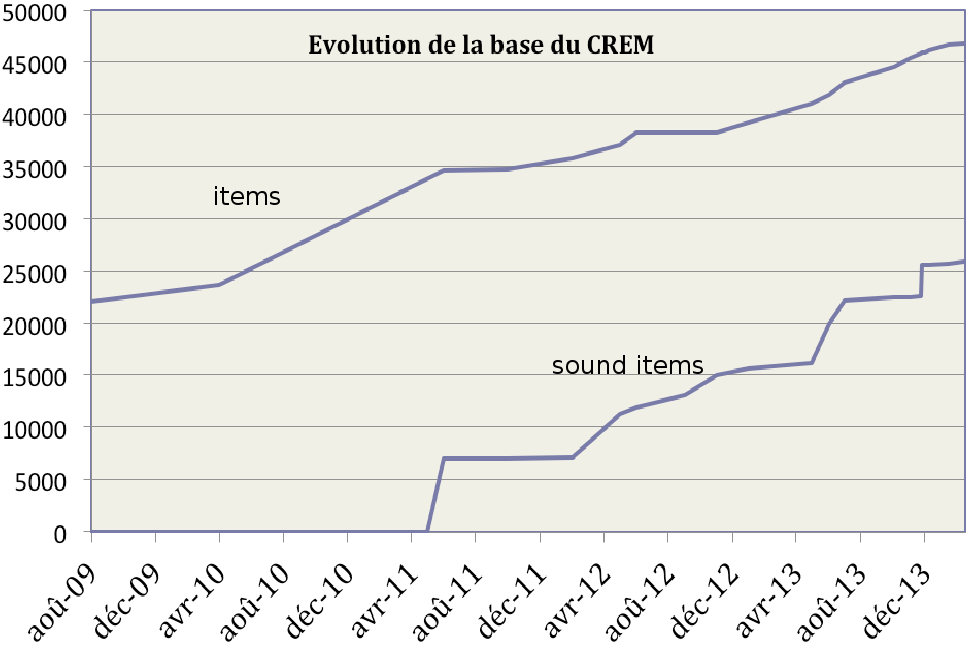
\includegraphics[width=0.8\textwidth]{img/crem_items.png}
%   \end{center}
% \end{frame}


\subsection{Technologies}
\frame{\frametitle{Technologies}

\begin{center}
\large{100\% 0pen Source!}
\end{center}

\begin{itemize}
 \item \chref{http://python.org}{Python} : smart object oriented language \\
 \item \chref{http://djangoproject.com}{Django} : high-level web MVC framework \\
 \item \chref{https://github.com/yomguy/TimeSide}{TimeSide} : open web audio processing framework 
 \item \chref{http://gstreamer.freedesktop.org/}{GStreamer} : open source multimedia framework
 \item MySQL, PostgreSQL, others : relational databases \\
 \item GNU / Linux : applications, libraries and kernel \\
\end{itemize}

}

\subsection{Features}
%\frame{\tableofcontents[currentsection]}
\frame{\frametitle{Key features}
      \begin{itemize}
      \item \alert{Pure HTML5} web user interface including dynamical forms
        and smart workflows
      \item \alert{On the fly} audio analyzing, transcoding and metadata
        embedding in various formats
      \item \alert{Social editing} with \alert{semantic ontologies}, smart workflows,
        realtime tools, human or automatic \alert{annotations and
        segmentations}
      \item \alert{User management} with individual desk, playlists, profiles
        and access rights
      \item \alert{High level search engine} (geolocation, instruments, ethnic groups, etc...)
      \item \alert{Data providers} : DublinCore, OAI-PMH, RSS, XML, JSON and other 
      \item \alert{Multi-language} support (now english and french)
      \end{itemize}
}


\section{Framework}

\subsection{Architecture}
\frame{\frametitle{Architecture}
    \begin{center}
    \pgfimage[width=8cm]{img/TM_arch}
    \end{center}
}



\section{Telemeta Web User Interface}
\begin{frame}\frametitle{Telemeta Web User Interface}
  \vspace{-0.25cm}
  \begin{center}
    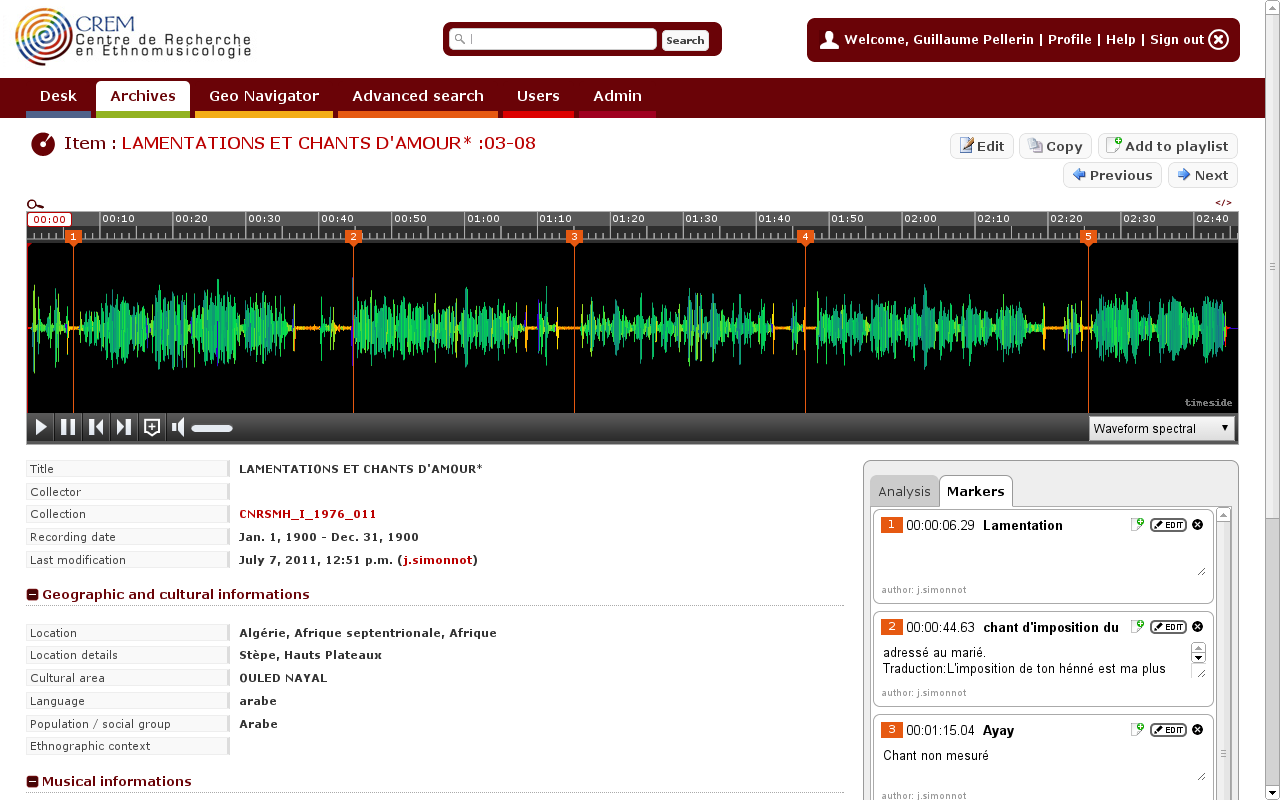
\includegraphics[width=12cm]{img/shots/telemeta_eng.png}
  \end{center}
  \tiny{\url{http://archives.crem-cnrs.fr/archives/items/CNRSMH_I_1976_011_003_08/}}
\end{frame}


\section{Related projects}
\frame{\tableofcontents[currentsection]}

\begin{frame}
 \frametitle{TimeSide : open web audio processing framework}%\scriptsize
\begin{block}{Server side - TimeSide Engine}
  \begin{itemize}
  \item \alert{Do} asynchronous and fast audio processing with Python,
  \item \alert{Decode} audio frames from ANY format into numpy arrays,
  \item \alert{Analyze} audio content with state-of-the-art audio feature extraction libraries (Aubio, Yaafe, Vamp (experimental),
  \item  \alert{Organize}, serialize and save analysis metadata through various formats,
  \item  \alert{Draw} various fancy waveforms, spectrograms and other cool graphers,
  \item  \alert{Transcode} audio data in various media formats and stream them through web apps,
  \end{itemize}
 
\end{block}
\begin{block}{Client side - TimeSide UI}
  \begin{itemize}
  \item   \alert{Playback} and  \alert{interact} on demand through a smart high-level HTML5 extensible player,
  \item   \alert{Index},  \alert{tag} and  \alert{organize semantic metadata} \\
(see \href{http://telemeta.org/}{Telemeta} which embeds TimeSide). 
\hfill $\vcenter{\hbox{\includegraphics[width=0.2\textwidth]{img/logo_telemeta_1-1.pdf}}}$
 % \begin{flushright}
 %   
\includegraphics[width=0.2\textwidth]{../../Common/img/logo_telemeta_1-1.pdf}\\
 %   \colorbox{yellow!50}{\textbf{\url{http://telemeta.org/}}}
  %\end{flushright}
  \end{itemize}
\end{block}
\end{frame}

\begin{frame}
  \frametitle{TimeSide - Architecture}
  \begin{center}
    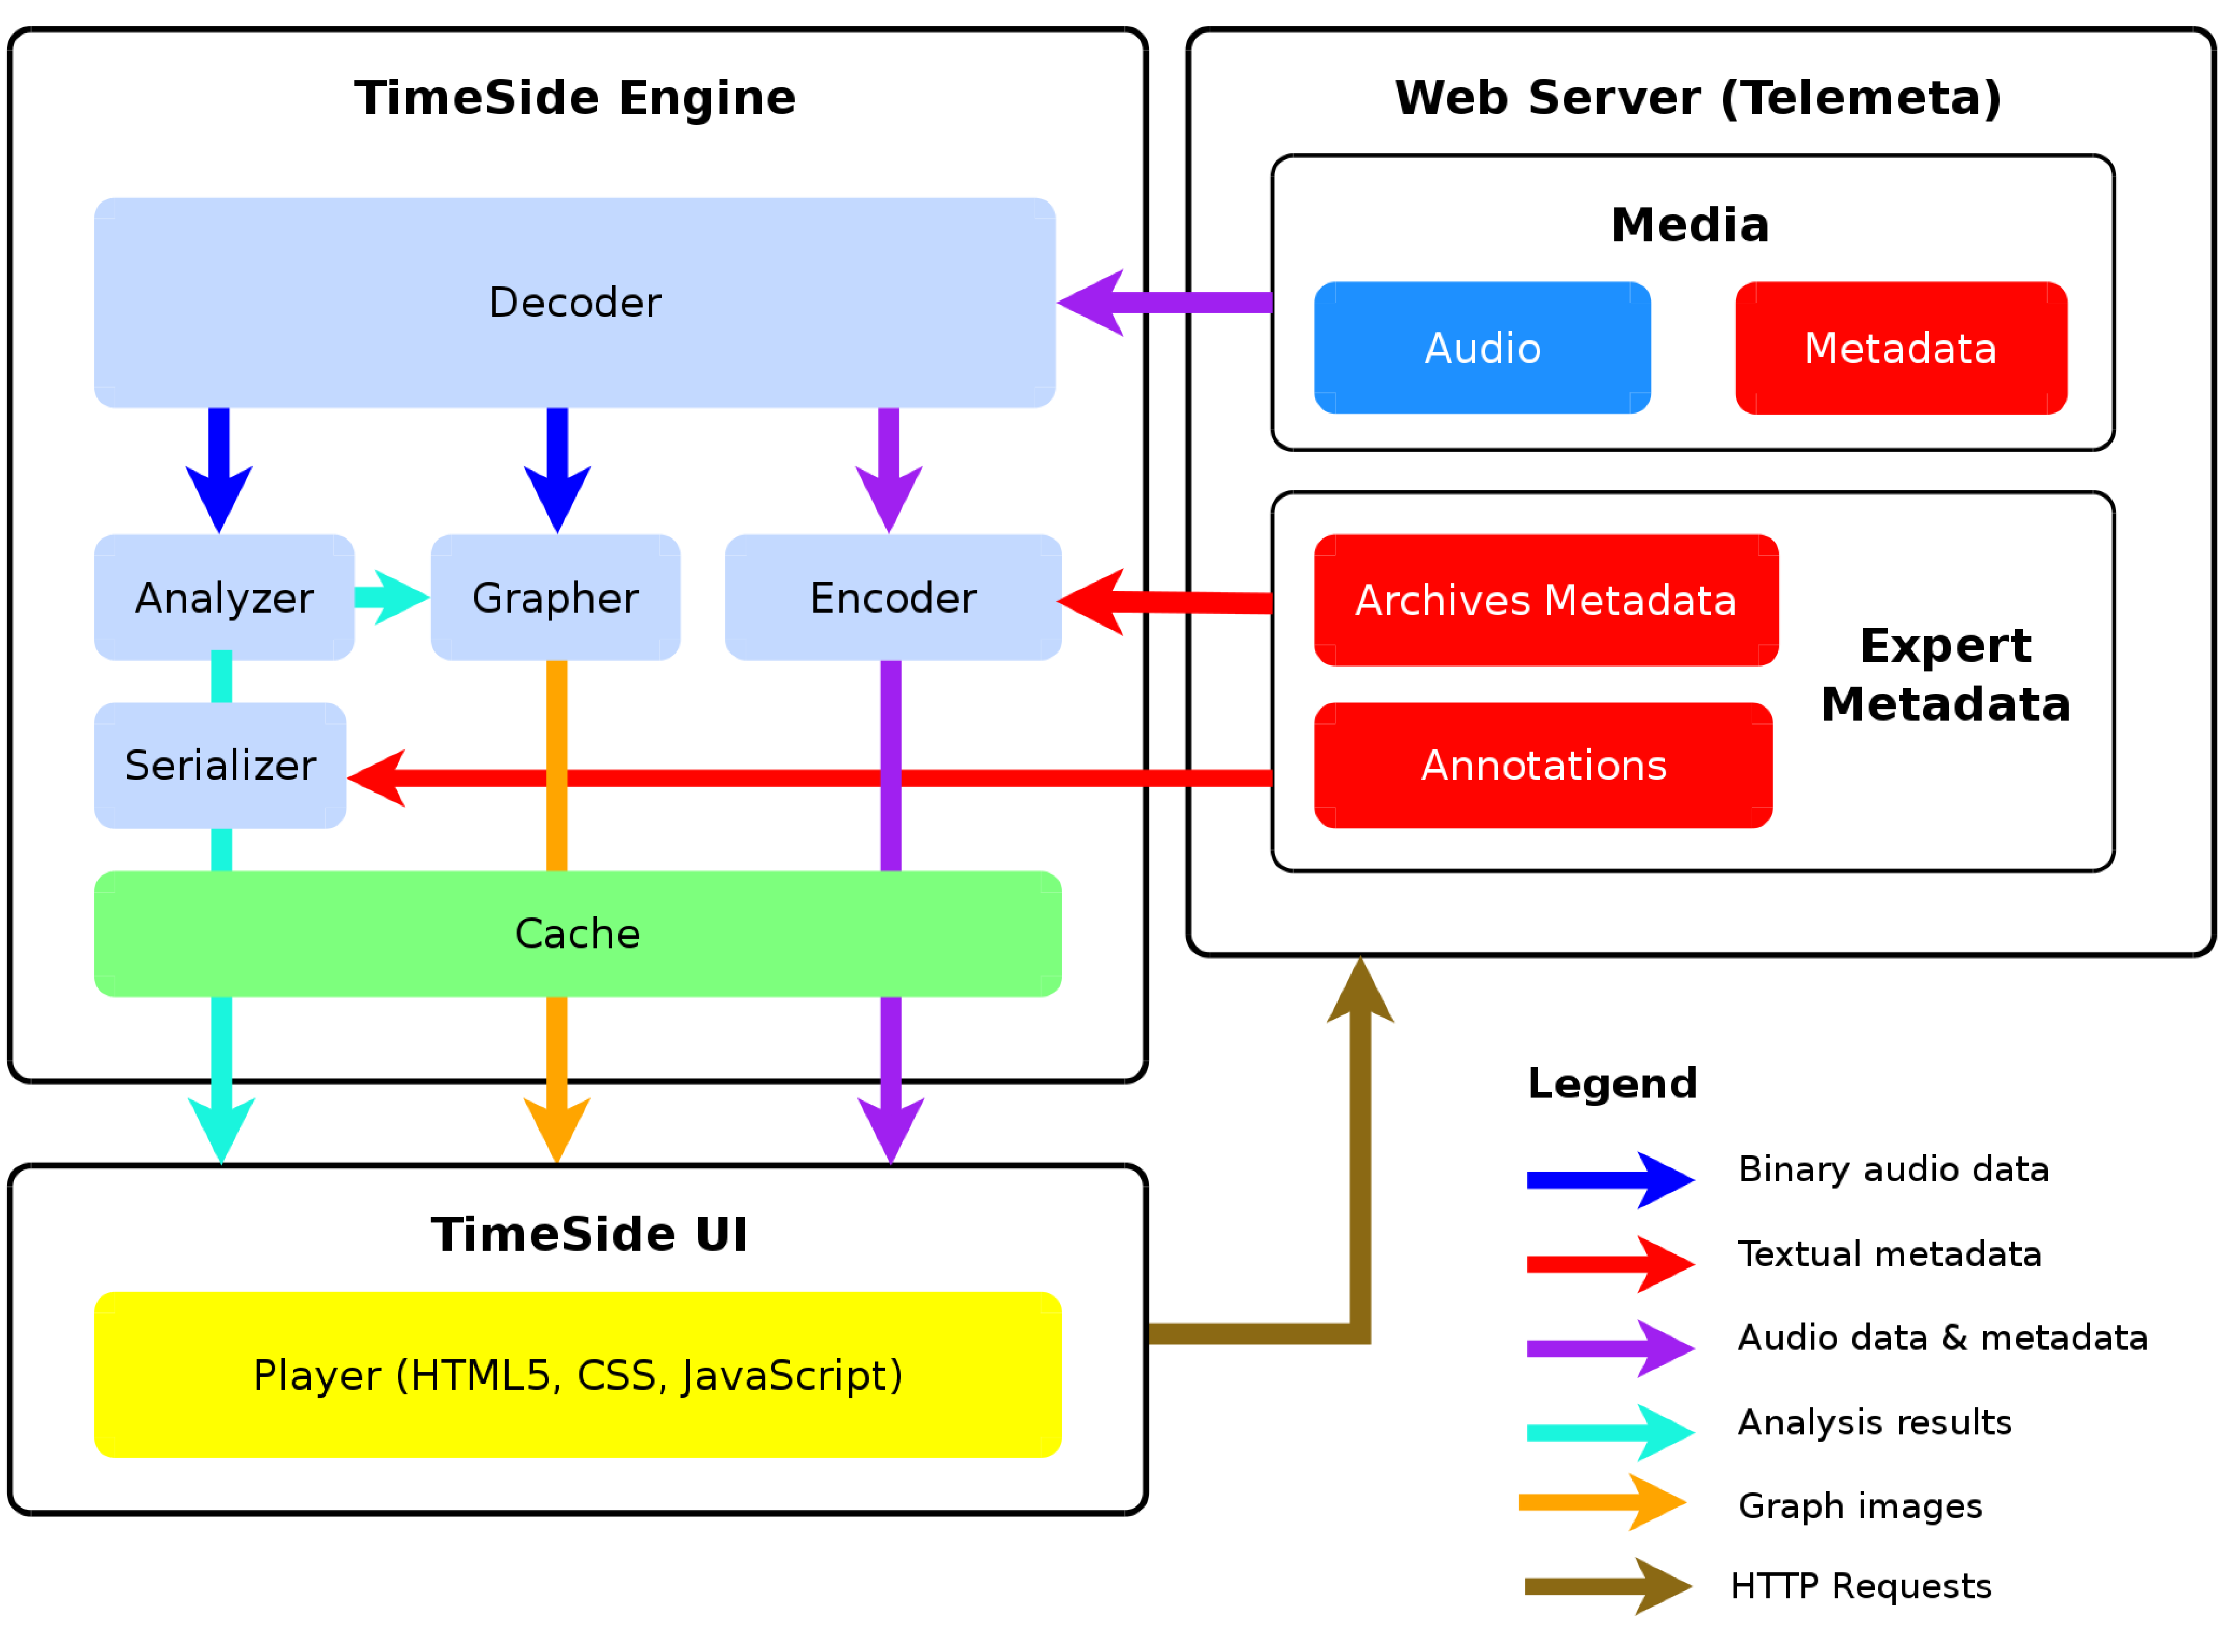
\includegraphics[width=0.8\textwidth]{img/timeside_schema_v3.pdf}
  \end{center}
\end{frame}

\begin{frame}
  \frametitle{TimeSide Engine}
  \begin{center}
    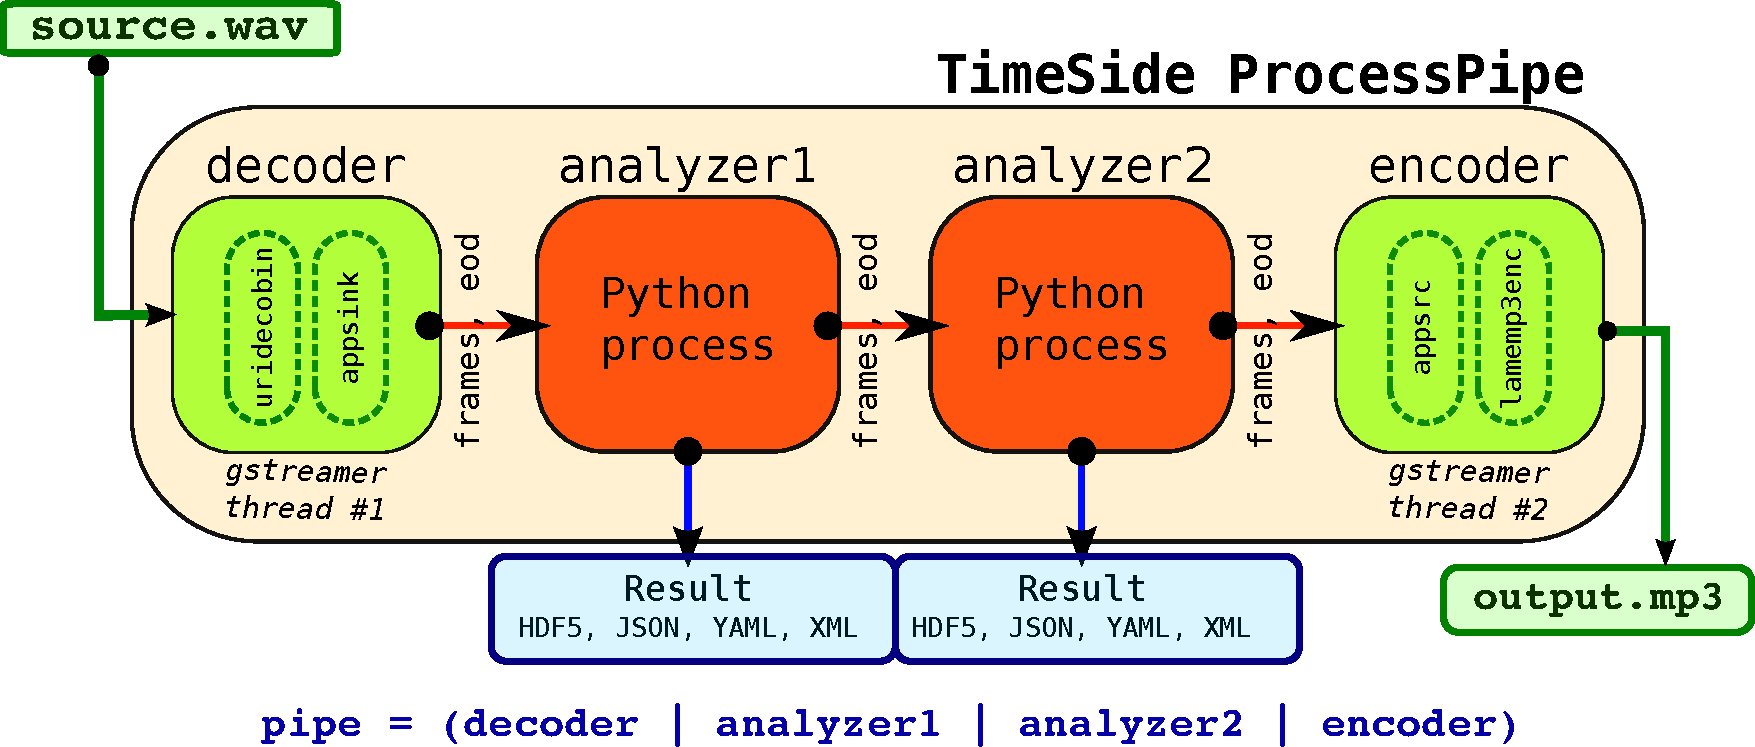
\includegraphics[width=0.95\textwidth]{img/TimeSide_pipe.pdf}
  \end{center}
  \begin{block}{Process Pipe}
    \begin{itemize}
    \item On-the-fly audio processing by simultaneous processors (decoder, encoders, analyzers, graphers)
    \item Use of \emph{Gstreamer} for audio decoding and encoding    \end{itemize}
  \end{block}
\end{frame}

\frame{\frametitle{The DIADEMS project}
\begin{itemize}
    \item \chref{http://www.irit.fr/recherches/SAMOVA/DIADEMS/fr/welcome/&cultureKey=en}{DIADEMS} : Description, Indexation, Access to Sound and Ethnomusicological Documents
    \item Granted by ANR : french national research agency (ANR-12-CORD-0022)     
    \item 3 years, 8 partners, 850 k\euro
    \item Apply and test MIR algorithms on large scale ethnomusicological data
    \item Define some high level interfaces to find new ways of explorations in large complex musical corpus
    \item New modes of collaboration between human science and computer science laboratories and researchers
    \item Define the \chref{http://files.parisson.com/telemeta/telemeta-doc/DIADEMS/thesaurus/Thesaurus/Thesaurus.html}{vocabulary} describing musical events in the usecase of ethnomusicilogy vs. signal processing
    \item \dchref{http://www.irit.fr/recherches/SAMOVA/DIADEMS/fr/welcome/}
    \item \dchref{http://diadems.telemeta.org}
\end{itemize}
}

\frame{\frametitle{DIADEMS - Partners}
\begin{itemize}
\item Sponsors:
\begin{itemize}
 \item CNRS
 \item Huma-Num (ex TGE Adonis)
 \item ANR
 \item CREM
 \item UPMC
 \item Parisson
\end{itemize}

\vspace{0.25cm}

\item Partners :
\begin{itemize}
\item IRIT (université Paul Sabatier, Toulouse 3)
\item LIMSI (universités Pierre et Marie Curie (UPMC, Paris 6) et Paris-Sud)
\item LAM (institut Jean Le Rond d'Alembert, UPMC)
\item LABRI (université de Bordeaux)
\item CREM (université Paris Ouest Nanterre La Défense)
\item LESC (université Paris Ouest Nanterre La Défense)
\item Museum d'Histoire Naturelle de Paris
\item Musée du Quai Branly
\end{itemize}

\end{itemize}

\begin{center}
\begin{columns}[c]
\column{2.5cm}
\begin{center}
\pgfimage[width=1cm]{img/logo-CNRS}\end{center}
\column{2.5cm}
\begin{center}
\pgfimage[width=2.5cm]{img/Logo-CREM-La.jpg}
\end{center}
\column{2.5cm}
\begin{center}
\pgfimage[width=2.5cm]{img/parisson_logo_200}\end{center}
\column{2cm}
\begin{center}
\pgfimage[width=1.2cm]{img/logo-mnhn}\end{center}
\end{columns}
\end{center}

}


\section{Development and contact informations}
%\frame{\tableofcontents[currentsection]}

\frame{\frametitle{Development}
\begin{block}{Links}
    \begin{itemize}
    \item \dchref{http://telemeta.org}
    \item \dchref{https://github.com/yomguy/Telemeta/}
    \item \dchref{https://github.com/yomguy/TimeSide/}
    \end{itemize}
\end{block}
\begin{block}{Team}
    \begin{itemize}
     \item Guillaume Pellerin
     \item Thomas Fillon
     \item Paul Brossier
     \item Riccardo Zaccarelli
     \item Maxime Lecoz
     \item David Doukan
    \end{itemize}
\end{block}
\begin{block}{Licence}
\chref{http://www.cecill.info/licences/Licence_CeCILL_V2.1-en.html}{CeCILL v2.1} (GPL v2 compatible) 
\end{block}
}


\frame{\frametitle{Development - Lessons from a 7 year old project}
\begin{itemize}
\item Simplicity is better than complexity (a Python developer rule)
\item Modularity is only accessible with a flexible language
\item Models and objects are more important than technologies
\item A good workflow is defined by the users themselves through feedback and revisions
\item Prototyping is a crucial part of the development process
\item A good platform should rely on standards, not on formats
\item The Open Source ecosystem gives some tremendous possibilities to scale a platform project
\end{itemize}
}

\frame{\frametitle{Development - TODO list}
\begin{block}{TimeSide}
    \begin{itemize}
    \item Tiny web server (django)
    \item Process task manager
    \item Full HTML5 zooming player (+ annotations, segmentations, etc..)
    \item Analyzer parameters (+ interface)
    \item Improve Vamp plugins support (Vamp python host ?)
    \item Add more automatic segmentation and classification tools to support various semantic ontologies (cf. thesaurus)
    \item Add more music analysis tools to support Ethnomusicological research
    \item Add automatic similarity analysis tools (inside a song or between sound items)
    \item Enhance analysis result displays to send to Telemeta
    \item \dchref{https://github.com/yomguy/TimeSide/issues}
    \end{itemize}
\end{block}
}


\frame{\frametitle{Development - TODO list}
\begin{block}{Telemeta}
    \begin{itemize}
    \item Update code to support Django new Class based views
    \item Rewrite geolocation services
    \item Public and enhanced user playlists
    \item Smart breadcrumbs 
    \item Better interactions with TimeSide
    \item Enhance user interface (full HTML 5 + web audio API)
        \begin{itemize}
            \item For annotations and segmentations in a collaborative manner
            \item Provide import capabilities and feedback loop between manual and automatic annotations
            \item Fancy displays of automatic analysis results (zoomable + synchronized with audio)
            \item Add a User interface to control and tune the analysis parameters
        \end{itemize}
    \item More documentation
    \item \dchref{http://telemeta.org/report/1}
    \end{itemize}
\end{block}
}



\frame{\frametitle{The End}
 \begin{center}
   \large{Thank you!}
   \vspace{0.25cm}
    \begin{block}{Links}
     \begin{itemize}
        \item \chref{http://telemeta.org}{telemeta.org}
        \item \chref{https://twitter.com/telemeta/}{@telemeta}
    \end{itemize}
    \end{block}
    \begin{block}{Contact}
    \begin{itemize}
    \item \chref{mailto:guillaume@parisson.com}{guillaume@parisson.com}
    \item \chref{https://twitter.com/yomguy/}{@yomguy}
    \item \chref{https://github.com/yomguy/}{github.com/yomguy/}
    \item \chref{https://plus.google.com/u/0/+GuillaumePellerin/posts}{+GuillaumePellerin}
    \item \chref{http://fr.linkedin.com/in/guillaumepellerin}{fr.linkedin.com/in/guillaumepellerin}
    \end{itemize}
     \end{block}
  \end{center}
}

% BONUS

\begin{frame}[fragile]
  \begin{block}{TimeSide - Github repository}
    \begin{center}\scriptsize
      \colorbox{yellow!50}{\bf \hskip3ex
        \url{https://github.com/yomguy/TimeSide/} \hskip3ex }
    \end{center}

  \begin{itemize}
  \item 3 main branches: master, dev, diadems 
  \end{itemize}
  \end{block}
  \begin{block}{Installation}
\url{https://github.com/yomguy/TimeSide\#install}
    \begin{itemize}
    \item Installation des dépendances :
\begin{lstlisting}[language=bash, basicstyle=\tiny]
$ echo "deb http://debian.parisson.com/debian/ stable main" |
$ sudo tee -a /etc/apt/sources.list 
$ echo "deb-src http://debian.parisson.com/debian/ stable main" | sudo tee -a /etc/apt/sources.list 
$ sudo apt-get update 
$ sudo apt-get install git 
$ sudo apt-get build-dep python-timeside
\end{lstlisting}

    \item Installation depuis le dépôt \emph{Github} :
\begin{lstlisting}[language=bash, basicstyle=\tiny]
$ git clone https://github.com/yomguy/TimeSide.git 
$ cd TimeSide 
$ git checkout dev 
$ export PYTHONPATH=$PYTHONPATH:`pwd` 
$ python tests/run_all_tests
\end{lstlisting}
\end{itemize}
\end{block}
\end{frame}


\end{document}